\documentclass{article}

\usepackage[utf8]{inputenc}  
\usepackage[T1]{fontenc}     
\usepackage{tikz}
\usetikzlibrary{shapes, positioning, arrows, calc}
\usetikzlibrary{decorations.pathreplacing}

\begin{document}

% Exemple tri

% 1ère étape : diviser

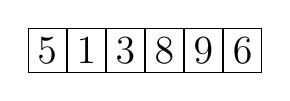
\begin{tikzpicture}
   \node [font=\sffamily\Large\bfseries, draw, anchor=center] (first) {$5$};
   \node [font=\sffamily\Large\bfseries, draw, anchor=center, right=0cm of first] (second) {$1$};
   \node [font=\sffamily\Large\bfseries, draw, anchor=center, right=0cm of second] (third) {$3$};
   \node [font=\sffamily\Large\bfseries, draw, anchor=center, right=0cm of third] (fourth) {$8$};
   \node [font=\sffamily\Large\bfseries, draw, anchor=center, right=0cm of fourth] (fifth) {$9$};
   \node [font=\sffamily\Large\bfseries, draw, anchor=center, right=0cm of fifth] (sixth) {$6$};
\end{tikzpicture}

\vspace{0.25cm}

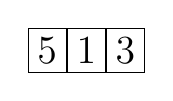
\begin{tikzpicture}
   \node [font=\sffamily\Large\bfseries, draw, anchor=center] (first) {$5$};
   \node [font=\sffamily\Large\bfseries, draw, anchor=center, right=0cm of first] (second) {$1$};
   \node [font=\sffamily\Large\bfseries, draw, anchor=center, right=0cm of second] (third) {$3$};
\end{tikzpicture}
\hspace{0.1cm}
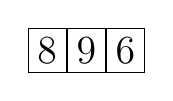
\begin{tikzpicture}
   \node [font=\sffamily\Large\bfseries, draw, anchor=center] (first) {$8$};
   \node [font=\sffamily\Large\bfseries, draw, anchor=center, right=0cm of first] (second) {$9$};
   \node [font=\sffamily\Large\bfseries, draw, anchor=center, right=0cm of second] (third) {$6$};
\end{tikzpicture}

\vspace{0.25cm}


\begin{tikzpicture}
   \node [font=\sffamily\Large\bfseries, draw, anchor=center] (first) {$5$};
\end{tikzpicture}
\hspace{0.1cm}
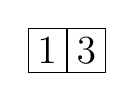
\begin{tikzpicture}
   \node [font=\sffamily\Large\bfseries, draw, anchor=center] (first) {$1$};
   \node [font=\sffamily\Large\bfseries, draw, anchor=center, right=0cm of first] (second) {$3$};
\end{tikzpicture}
\hspace{0.1cm}

\begin{tikzpicture}
   \node [font=\sffamily\Large\bfseries, draw, anchor=center] (first) {$8$};
\end{tikzpicture}
\hspace{0.1cm}
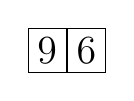
\begin{tikzpicture}
   \node [font=\sffamily\Large\bfseries, draw, anchor=center] (first) {$9$};
   \node [font=\sffamily\Large\bfseries, draw, anchor=center, right=0cm of first] (second) {$6$};
\end{tikzpicture}

\vspace{0.25cm}

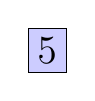
\begin{tikzpicture}
   \node [fill=blue!20, font=\sffamily\Large\bfseries, draw, anchor=center] (first) {$5$};
\end{tikzpicture}
\hspace{0.1cm}

\begin{tikzpicture}
   \node [fill=blue!20, font=\sffamily\Large\bfseries, draw, anchor=center] (first) {$1$};
\end{tikzpicture}
\hspace{0.1cm}
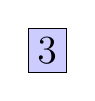
\begin{tikzpicture}
   \node [fill=blue!20, font=\sffamily\Large\bfseries, draw, anchor=center] (first) {$3$};
\end{tikzpicture}
\hspace{0.1cm}
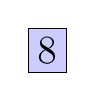
\begin{tikzpicture}
   \node [fill=blue!20, font=\sffamily\Large\bfseries, draw, anchor=center] (first) {$8$};
\end{tikzpicture}
\hspace{0.1cm}
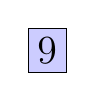
\begin{tikzpicture}
   \node [fill=blue!20, font=\sffamily\Large\bfseries, draw, anchor=center] (first) {$9$};
\end{tikzpicture}
\hspace{0.1cm}
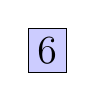
\begin{tikzpicture}
   \node [fill=blue!20, font=\sffamily\Large\bfseries, draw, anchor=center] (first) {$6$};
\end{tikzpicture}
\hspace{0.1cm}

% 2ème étape : fusionner

\vspace{1cm}

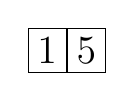
\begin{tikzpicture}
   \node [font=\sffamily\Large\bfseries, draw, anchor=center] (first) {$1$};
   \node [font=\sffamily\Large\bfseries, draw, anchor=center, right=0cm of first] (second) {$5$};
\end{tikzpicture}
\hspace{0.1cm}
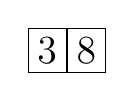
\begin{tikzpicture}
   \node [font=\sffamily\Large\bfseries, draw, anchor=center] (first) {$3$};
   \node [font=\sffamily\Large\bfseries, draw, anchor=center, right=0cm of first] (second) {$8$};
\end{tikzpicture}
\hspace{0.1cm}
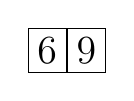
\begin{tikzpicture}
   \node [font=\sffamily\Large\bfseries, draw, anchor=center] (first) {$6$};
   \node [font=\sffamily\Large\bfseries, draw, anchor=center, right=0cm of first] (second) {$9$};
\end{tikzpicture}
\hspace{0.1cm}

\vspace{0.25cm}

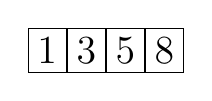
\begin{tikzpicture}
   \node [font=\sffamily\Large\bfseries, draw, anchor=center] (first) {$1$};
   \node [font=\sffamily\Large\bfseries, draw, anchor=center, right=0cm of first] (second) {$3$};
   \node [font=\sffamily\Large\bfseries, draw, anchor=center, right=0cm of second] (third) {$5$};
   \node [font=\sffamily\Large\bfseries, draw, anchor=center, right=0cm of third] (fourth) {$8$};
\end{tikzpicture}
\hspace{0.1cm}
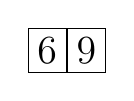
\begin{tikzpicture}
   \node [font=\sffamily\Large\bfseries, draw, anchor=center] (first) {$6$};
   \node [font=\sffamily\Large\bfseries, draw, anchor=center, right=0cm of first] (second) {$9$};
\end{tikzpicture}
\hspace{0.1cm}

\vspace{0.25cm}

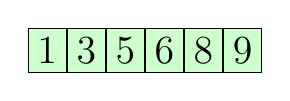
\begin{tikzpicture}
   \node [fill=green!20, font=\sffamily\Large\bfseries, draw, anchor=center] (first) {$1$};
   \node [fill=green!20, font=\sffamily\Large\bfseries, draw, anchor=center, right=0cm of first] (second) {$3$};
   \node [fill=green!20, font=\sffamily\Large\bfseries, draw, anchor=center, right=0cm of second] (third) {$5$};
   \node [fill=green!20, font=\sffamily\Large\bfseries, draw, anchor=center, right=0cm of third] (fourth) {$6$};
   \node [fill=green!20, font=\sffamily\Large\bfseries, draw, anchor=center, right=0cm of fourth] (fifth) {$8$};
   \node [fill=green!20, font=\sffamily\Large\bfseries, draw, anchor=center, right=0cm of fifth] (sixth) {$9$};
\end{tikzpicture}

\end{document}
